\chapter{Implementation PUT IN OWN FILE}

\section{User interface}
\subsection{Main Display}
\label{mainimp}
The main display represents the general interface is displayed to the user. This is where the algorithms visual representation will be presented, as well as providing the location of the user interaction elements enabling modification of the algorithms parameters. This interface is a result of the contents of the DisplayFrame Class and its contents. The design for this view is generally as described in section \ref{ssec:mainUI}, appendix B, however, there has been a slight modification to this proposed design.

\begin{figure}[H]
\centering
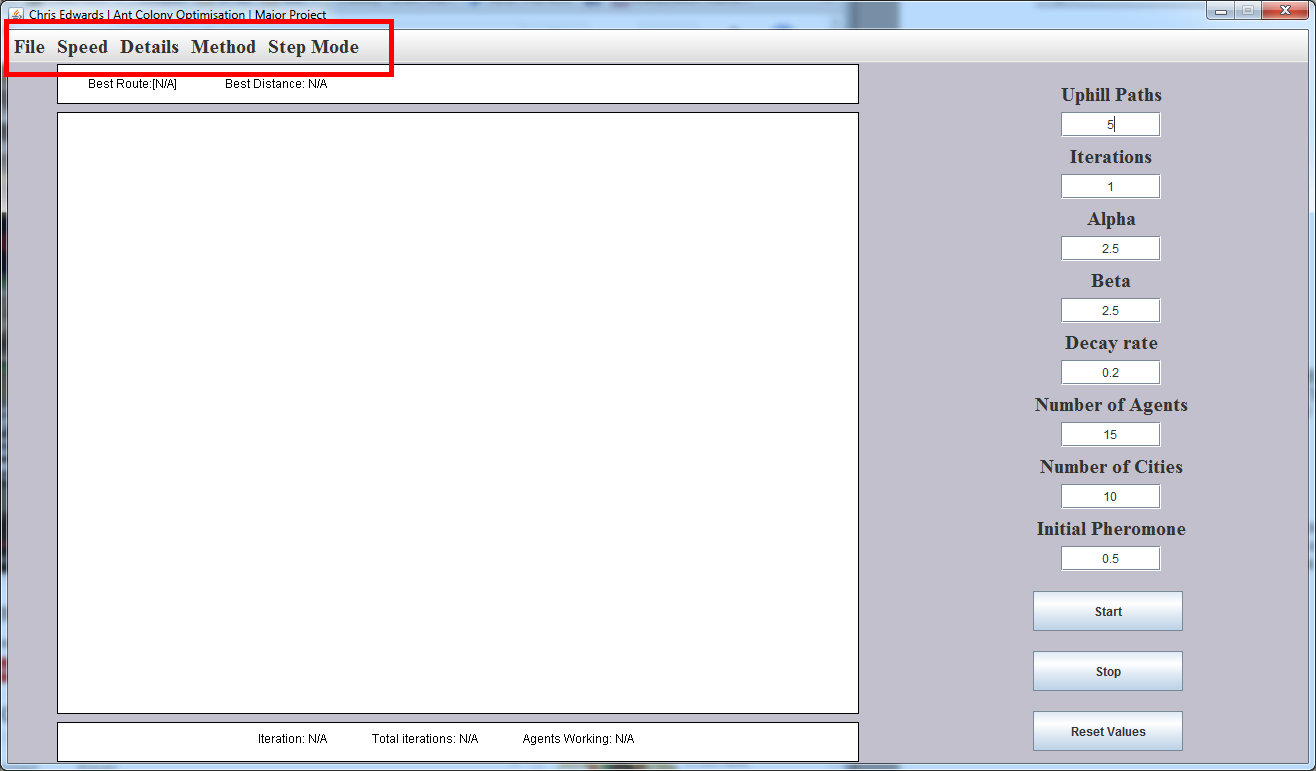
\includegraphics[scale=0.35]{Images/chapter4/displayFrame}
\caption{Implementation of the proposed user interface. The contents of the red polygon highlights the additional features not present in the initial design.}
\label{fig:displayFrameImp}
\end{figure}

The additional features highlighted by the red polygon in figure \ref{fig:displayFrameImp} represent the features which were not initially designed. These features are represented in a separate location to the control panel (right hand side of figure \ref{fig:displayFrameImp}) as there is no logical connection between the menu bar features, and the modification of the algorithm parameters. The author opted to use a menu bar to control the access to these features as the vast majority of users will recognise what a menu bar is, and understand how to interact with such elements. 

The different elements contained in this menu bar relate to general system interactions. The File option enables the user to either load, or save a configuration to a specified file. The Speed option enables the user to change the Thread speed, which will directly change the algorithms rate of execution. The Details menu is used to control access to any additional views. The views which can be access here are; the Uphill Viewer (section \ref{uphillview}), The City Detail View (section \ref{deetzlview}) and the Equation Viewer (section \ref{eqnlview}). In addition to the access of these extra views, the Detail menu also enables the user to disable and enable uphill routes \Large REFERENCE UPHILL ROUTES GENERATION ALGORITHM PSEUDO CODE \normalsize to be generated for current problem. The Method option enables the user to select the current algorithm type from a list of implement algorithm types. Currently the author has implemented a Basic Ant System and an Elitist Ant system so the user can switch between these algorithm types. The Step Mode menu enables the user to enable or disable the step mode functionality. When enabled, step mode will allow the user to step through the algorithms execution at their own pace without the application automatically solving the problem.

\Large TALK ABOVE MOVE FUNCTIONS, AGLORITHMS ABOVE INC CANVAS PAINTING, STEP BASED INTERATION, SWING WORKER TO STOP UI FREEZING, REASON FOR THE NEW PHERO VARAIBALE IN THE PHEROMONE CLASS, DATA STRUCTURES, WHY LINKED LIST WAS USED FOR BEST ROUTES, LINEAR INTERPOLATION, ALSO MENTION SCALE FACTOR (EVERYTHING IS X20) MAYBE TALK ABOUT PHEROMONE DECAY MODELLING USING ALPHA VALUES \normalsize


The implementation should look at any issues you encountered as you tried to implement your design. During the work, you might have found that elements of your design were unnecessary or overly complex; perhaps third party libraries were available that simplified some of the functions that you intended to implement. If things were easier in some areas, then how did you adapt your project to take account of your findings?

It is more likely that things were more complex than you first thought. In particular, were there any problems or difficulties that you found during implementation that you had to address? Did such problems simply delay you or were they more significant? 

You can conclude this section by reviewing the end of the implementation stage against the planned requirements. 

\chapter{Testing PUT THIS IN OWN FILE}

Detailed descriptions of every test case are definitely not what is required here. What is important is to show that you adopted a sensible strategy that was, in principle, capable of testing the system adequately even if you did not have the time to test the system fully.

Have you tested your system on �real users�? For example, if your system is supposed to solve a problem for a business, then it would be appropriate to present your approach to involve the users in the testing process and to record the results that you obtained. Depending on the level of detail, it is likely that you would put any detailed results in an appendix.

The following sections indicate some areas you might include. Other sections may be more appropriate to your project. 

\section{Overall Approach to Testing}

\section{Automated Testing}

\subsection{Unit Tests}

\subsection{User Interface Testing}

\subsection{Stress Testing}

\subsection{Other types of testing}

\section{Integration Testing}

\section{User Testing}

\chapter{Evaluation}

Examiners expect to find in your dissertation a section addressing such questions as:

\begin{itemize}
   \item Were the requirements correctly identified? 
   \item Were the design decisions correct?
   \item Could a more suitable set of tools have been chosen?
   \item How well did the software meet the needs of those who were expecting to use it?
   \item How well were any other project aims achieved?
   \item If you were starting again, what would you do differently?
\end{itemize}

Such material is regarded as an important part of the dissertation; it should demonstrate that you are capable not only of carrying out a piece of work but also of thinking critically about how you did it and how you might have done it better. This is seen as an important part of an honours degree. 

There will be good things and room for improvement with any project. As you write this section, identify and discuss the parts of the work that went well and also consider ways in which the work could be improved. 

Review the discussion on the Evaluation section from the lectures. A recording is available on Blackboard. 
